\section{Diffusion/mean square displacement}
\todod{Diffusion normal to and parallel to surface?}
\todob{Plot of $r^2$ for 200 and 40 states to argue for origo move?}

% bulk diff in Ref \#1 = 0.202034846318
%   N = mean(47577, 47524, 47555, 47552, 47559) = 
% bulk diff in Ref \#2 = 0.178684448075
%   N = mean(50280, 50284, 50291, 50275, 50321)

% bulk diff in Rough \#1 = 0.197721045372      
%   N = mean(4271, 4279, 4252, 4294, 4284)
% bulk diff in Rough \#2 = 0.208658027239  
%   N = mean(3414, 3396, 3419, 3431, 3393)


To produce these results we have averaged over 200 states, with 100 timesteps of 20.67 md units between each timestep ($\sim 0.5$ picoseconds\hl{???}), divided into 5 non-overlapping origos, with 40 states per origo.

We first look at the diffusion as function of distance to the silica matrix in the four reference systems, which we have plotted in \cref{fig:diffusion_reference_systems}. We see that the diffusion constant, $D$, has similar quantitative behaviour as we move further from the silica matrix in all four reference systems, but that the actual $D$ is different in each system. The two systems with 86 \AA\ wide flat pores have diffusion constants that differ by around 10-30\%, even though those two systems should be pretty similar. The main difference between those two systems is the density, as we saw in \cref{sec:results_density}. We have listed the bulk $D$ in \cref{tab:bulk_water_diffusion}, and we see that the bulk diffusion for the two reference systems with 86 \AA\ wide flat pores is {0.202 \AA$^2$/ps}, while system \#2 has {0.179 \AA$^2$/ps}, with a difference of {13 \%}.
%
%
% \begin{figure}[htpb]%
%     \centering%
%     \includesvg[width=0.6\textwidth, svgpath=./images/diffusion/]{diffusion_constant_move_origin_reference01}%
%     \caption{%
%         Diffusion constant as function of distance to silica matrix for all four reference systems (flat fractures). The solid lines are for the two systems with 86 \AA\ wide fractures, and the dashed lines for narrow fractures of 14.4 and 28.8 \AA. \hl{FINISH CAPTION}. %
%         \label{fig:diffusion_reference_systems}%
%     }%
% \end{figure}%

In \cref{fig:diffusion_rough_systems} we have plotted the diffusion constant %as function of distance from the silica matrix 
for the four random fracture systems, ``rough \#1'' through 4. We again see a quantitative similar behaviour, and we see that all systems except the 14.4 \AA\ narrow fracture (``rough \#3'') have very similar diffusion constants. In \cref{tab:bulk_water_diffusion} see that the bulk diffusion constants in the two regular random fractures (\#1 and \#2) are similar, with a difference of {6 \%}. We also see that the $D$ for water at 7-10 \AA\ from the silica matrix is close to the bulk constant for these two systems.
\todoao{More about diffusion?}
%
% \begin{figure}[htpb]%
%     \centering%
%     \includesvg[width=0.6\textwidth, svgpath=./images/diffusion/]{diffusion_constant_move_origin_rough01}%
%     \caption{%
%         Diffusion constant as function of distance to silica matrix for all four random/rough fractures. \hl{FINISH CAPTION}. %
%         \label{fig:diffusion_rough_systems}%
%     }%
% \end{figure}%
%
%
\begin{figure}[htpb]%
% \centering%
\setlength{\myfigwidth}{0.58\textwidth}%
\makebox[\textwidth][c]{ % to center figures below that are wider than \textwidth
    \begin{minipage}[t]{\myfigwidth}%
        \captionsetup{width=0.925\textwidth}%
        \centering%
        \includesvg[width=\textwidth, svgpath=./images/diffusion/]{diffusion_constant_move_origin_reference01}%
        \caption{%
            Diffusion constant as function of distance to silica matrix for all four reference systems (flat pores). The solid lines are for the two systems with 86 \AA\ wide pores, and the dashed lines for narrow fractures of 14.4 and 28.8 \AA. \hl{FINISH CAPTION}. %
            \label{fig:diffusion_reference_systems}%
        }%
    \end{minipage}%
    \hfill%
    \begin{minipage}[t]{\myfigwidth}% % change "b" to "t" to anchor top instead of bottom
        \captionsetup{width=0.925\textwidth}% % minipage defines a \textwidth for it's own, so we have to repeat this command inside the minipage
        \centering%
        \includesvg[width=\textwidth, svgpath=./images/diffusion/]{diffusion_constant_move_origin_rough01}%
        \caption{%
            Diffusion constant as function of distance to silica matrix for all four random rough fractures. Solid lines are for regular random fractures, and dashed lines for narrow fractures with uniform width of 14.4 and 28.8 \AA. \hl{FINISH CAPTION}. %
            \label{fig:diffusion_rough_systems}%
        }%
    \end{minipage}%
}
\end{figure}%

% \begin{figure}[htpb]%
%     \centering%
%     {
%         \newcommand{\f}{\footnotesize}
%         \includesvg[width=0.7\textwidth, svgpath=./images/diffusion/]{diffusion01}%
%     }
%     \caption{%
%         Diffusion. \hl{Make new figure using new diffusion program}. %
% %         \label{fig:cell_lists}%
%     }%
% \end{figure}%

% \begin{figure}[htpb]%
%     \centering%
%     {
%         \newcommand{\f}{\footnotesize}%
%         \includesvg[width=0.7\textwidth, svgpath=./images/diffusion/]{diffusion_constant02}%
%     }
%     \caption{%
%         Diffusion. \hl{Make new figure using new diffusion program} \hl{FINISH CAPTION}. %
% %         \label{fig:cell_lists}%
%     }%
% \end{figure}%

The bulk diffusion constants have been estimated in the two reference systems with 86 \AA\ wide flat pores (reference \#1 and \#2), and in rough system \#1 and \#2, by measuring $D$ for all water molecules further away from the silica matrix than 10 \AA. The results can be seen in \cref{tab:bulk_water_diffusion}. The other four systems have very narrow pores and fractures, with most of the water molecules closer to the silica matrix than 10 \AA\, so we haven't measured the bulk diffusion in those systems, and we don't expect much of the water to have bulk behaviour\todobo{explain this better?}.
%
\begin{table}[!htb]%
    \centering%
    \begin{tabular}{l|cc}%
        \textit{System} & Bulk $D$ [\AA$^2$/ps] & N    \\\hline
        Reference \#1   & 0.202                 & 48k  \\ % 0.202034846318
        Reference \#2   & 0.179                 & 50k  \\ % 0.178684448075
        Rough \#1       & 0.198                 & 4.3k \\ % 0.197721045372
        Rough \#2       & 0.209                 & 3.4k \\ % 0.208658027239
    \end{tabular}%
    \vspace{8pt}%
    \caption{%
        Bulk diffusion constant for water (for $r>10$ \AA), and the number of water molecules used in the calculations. %
        \label{tab:bulk_water_diffusion}%
    }%
\end{table}

\begin{figure}[htpb]%
% \centering%
\setlength{\myfigwidth}{0.58\textwidth}%
\makebox[\textwidth][c]{ % to center figures below that are wider than \textwidth
    \begin{minipage}[t]{\myfigwidth}%
        \captionsetup{width=0.925\textwidth}%
        \centering%
        \includesvg[width=\textwidth, svgpath=./images/diffusion/]{diffusion_constant_move_origin_normal01}%
        \caption{%
            Diffusion for random rough fractures and reference systems. \hl{reference figure or remove} \hl{FINISH CAPTION}. %
    %         \label{fig:cell_lists}%
        }%
    \end{minipage}%
    \hfill%
    \begin{minipage}[t]{\myfigwidth}% % change "b" to "t" to anchor top instead of bottom
        \captionsetup{width=0.925\textwidth}% % minipage defines a \textwidth for it's own, so we have to repeat this command inside the minipage
        \centering%
        \includesvg[width=\textwidth, svgpath=./images/diffusion/]{diffusion_constant_move_origin_narrow01}%
        \caption{%
            Diffusion for random narrow fractures and reference systems. \hl{reference figure or remove} \hl{FINISH CAPTION}. %
    %         \label{fig:cell_lists}%
        }%
    \end{minipage}%
}
\end{figure}%

% \begin{figure}[htpb]%
%     \centering%
%     \includesvg[width=0.8\textwidth, svgpath=./images/diffusion/]{diffusion_constant_move_origin_normal01}%
%     \caption{%
%         Diffusion for random rough fractures and reference systems. \hl{reference figure or remove} \hl{FINISH CAPTION}. %
% %         \label{fig:cell_lists}%
%     }%
% \end{figure}%
% 
% \begin{figure}[htpb]%
%     \centering%
%     \includesvg[width=0.8\textwidth, svgpath=./images/diffusion/]{diffusion_constant_move_origin_narrow01}%
%     \caption{%
%         Diffusion for random narrow fractures and reference systems. \hl{reference figure or remove} \hl{FINISH CAPTION}. %
% %         \label{fig:cell_lists}%
%     }%
% \end{figure}%

% \begin{figure}[htpb]%
%     \centering%
%     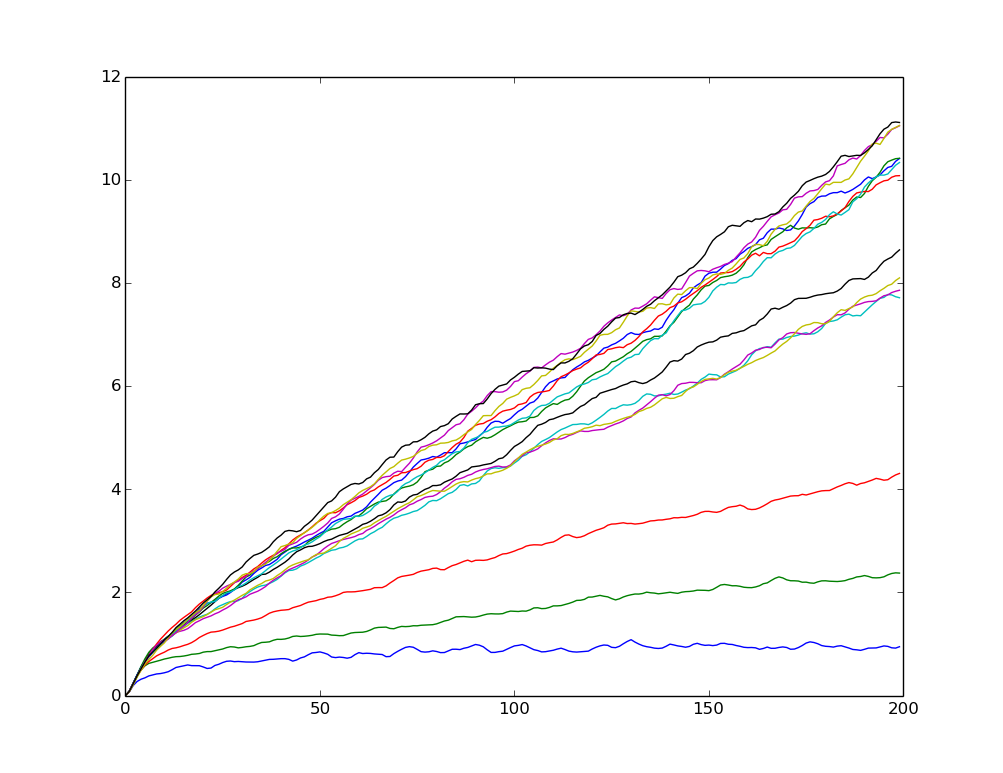
\includegraphics[width=0.5\textwidth]{images/diffusion/mean_square_displacement_interesting.png}%
%     \caption{%
%         Something interesting (msd stops increasing for a couple of angstrom near 4.5-5, 5-5.5, 5.5-6.0) \hl{reference figure or remove} \hl{FINISH CAPTION}. %
% %         \label{fig:cell_lists}%
%     }%
% \end{figure}%

% \begin{figure}[htpb]%
%     \centering%
%     \setlength{\myfigwidth}{0.49\textwidth}%
% %     \setlength{\mycaptionwidth}{0.3\textwidth}%
% %
%     \begin{subfigure}[b]{\myfigwidth}%
%         \includesvg[width=\textwidth, svgpath=./images/diffusion/]{diffusion_constant_move_origin01}%
%         \caption{%
%             Diffusion. \hl{FINISH CAPTION}. %
%     %         \label{fig:cell_lists}%
%         }%
%     \end{subfigure}%
%     \hfill%
%     \begin{subfigure}[b]{\myfigwidth}%
%         \includesvg[width=\textwidth, svgpath=./images/diffusion/]{diffusion_constant_move_origin02}%
%         \caption{%
%             Diffusion. \hl{FINISH CAPTION}. %
%     %         \label{fig:cell_lists}%
%         }%
%     \end{subfigure}%
%     \caption{%
%         rough\_fracture\_01\_abel - ``Rough fracture \#1'' \hl{Caption} %
%         \label{fig:renderings_rough_fracture01_abel}%
%     }%
% \end{figure}%